% 論文の構成
% 表紙
% 概要
% 目次
% 第1章(緒論 )
% 第2章(アプリケーション )
% 第3章(システム制御 )
% 第4章(結論)
% 謝辞
% 参考文献
% 付録

%卒業論文用雛形
\documentclass[a4j,12pt,oneside,openany]{jsbook}
% 英語なら以下を使う.
%\documentclass[a4j,12pt,oneside,openany,english]{jsbook}

\usepackage[dvipdfmx]{graphicx}
\usepackage{amssymb}
\usepackage{amsmath}
\usepackage{latexsym}

%jsbook を report っぽくするスタイルファイル
\usepackage{book2report}
%定理,補題,系,例題,証明などや英語用の定義がされています.
%自分なりにいじってください.
\usepackage{thesis}
% 具体的には以下のように定義されています.
% 英語の定理環境
%  \newtheorem{theorem}{Theorem}[chapter]
%  \newtheorem{lemma}{Lemma}[chapter]
%  \newtheorem{proposition}{Proposition}[chapter]
%  \newtheorem{corollary}{Corollary}[chapter]
%  \newtheorem{definition}{Definition}[chapter]
%  \newtheorem{example}{Example}[chapter]
%  \newtheorem{proof}{Proof}
% 日本語の定理環境
%  \newtheorem{theorem}{定理}[chapter]
%  \newtheorem{lemma}{補題}[chapter]
%  \newtheorem{proposition}{命題}[chapter]
%  \newtheorem{corollary}{系}[chapter]
%  \newtheorem{definition}{定義}[chapter]
%  \newtheorem{example}{例}[chapter]
%  \newtheorem{proof}{証明}
% 証明には番号をつけず,最後は Box で終わります.

% 英語で,見出しのフォントが気に入らなかったら
%\renewcommand{\headfont}{\bfseries}

% ページ数が少ないときはここを大きくしてごまかそう!!効果絶大!!
\renewcommand{\baselinestretch}{1.0}

\begin{document}

\renewcommand{\include}[1]{}
\renewcommand\documentclass[2][]{}

% 表紙
%卒業論文用雛形
\documentclass[a4j,12pt,oneside,openany]{jsbook}
% 英語なら以下を使う.
%\documentclass[a4j,12pt,oneside,openany,english]{jsbook}

\usepackage[dvipdfmx]{graphicx}
\usepackage{amssymb}
\usepackage{amsmath}
\usepackage{latexsym}

%jsbook を report っぽくするスタイルファイル
\usepackage{book2report}
%定理,補題,系,例題,証明などや英語用の定義がされています.
%自分なりにいじってください.
\usepackage{thesis}
% 具体的には以下のように定義されています.
% 英語の定理環境
%  \newtheorem{theorem}{Theorem}[chapter]
%  \newtheorem{lemma}{Lemma}[chapter]
%  \newtheorem{proposition}{Proposition}[chapter]
%  \newtheorem{corollary}{Corollary}[chapter]
%  \newtheorem{definition}{Definition}[chapter]
%  \newtheorem{example}{Example}[chapter]
%  \newtheorem{proof}{Proof}
% 日本語の定理環境
%  \newtheorem{theorem}{定理}[chapter]
%  \newtheorem{lemma}{補題}[chapter]
%  \newtheorem{proposition}{命題}[chapter]
%  \newtheorem{corollary}{系}[chapter]
%  \newtheorem{definition}{定義}[chapter]
%  \newtheorem{example}{例}[chapter]
%  \newtheorem{proof}{証明}
% 証明には番号をつけず,最後は Box で終わります.

% 英語で,見出しのフォントが気に入らなかったら
%\renewcommand{\headfont}{\bfseries}

% ページ数が少ないときはここを大きくしてごまかそう!!効果絶大!!
\renewcommand{\baselinestretch}{1.0}

\begin{document}

%%%%%%%%%%%% 題目 %%%%%%%%%%%%%%%%%%%%%%%%%%%%%%%%%%%%%%%%%%%%%%%%%%%%%%%
%%%%%%%%%%%% ここも適当に変えてもいいと思う %%%%%%%%%%%%%%%%%%%%%%%%%%%%%%%%%
\thispagestyle{empty}
\begin{center}
\vspace*{5mm}
{\Huge {\textbf{修} \hspace{12pt} \textbf{士} \hspace{12pt} \textbf{学} \hspace{12pt} \textbf{位} \hspace{12pt} \textbf{論} \hspace{12pt} \textbf{文}}}\\
\vspace{2cm}
{\Large 題\hspace{8mm}目}\\
\vspace{1cm}
\underline{\LARGE{タクシー乗務員のための}} \\
\vspace{0.5cm}
\underline{\LARGE{運転支援アプリケーションの設計}} \\
\vspace{12mm}
{\large 指 導 教 員}\\
\vspace{6mm}
\underline{\Large 潮 俊光 教 授}\\
\vspace{8mm}
{\large 報 告 者}\\
\vspace{6mm}
\underline{\Large 広本 将基}\\
\vspace{10mm}
{\Large 平成29年2月8日}\\
\vspace{14mm}
{\Large 大阪大学基礎工学研究科\\システム創成専攻社会システム数理領域\\博士前期課程}\\
\end{center}
\clearpage
\setcounter{page}{0}

\end{document}

\frontmatter

% 概要
%卒業論文用雛形
\documentclass[a4j,12pt,oneside,openany]{jsbook}
% 英語なら以下を使う.
%\documentclass[a4j,12pt,oneside,openany,english]{jsbook}

\usepackage[dvipdfmx]{graphicx}
\usepackage{amssymb}
\usepackage{amsmath}
\usepackage{latexsym}

%jsbook を report っぽくするスタイルファイル
\usepackage{book2report}
%定理,補題,系,例題,証明などや英語用の定義がされています.
%自分なりにいじってください.
\usepackage{thesis}
% 具体的には以下のように定義されています.
% 英語の定理環境
%  \newtheorem{theorem}{Theorem}[chapter]
%  \newtheorem{lemma}{Lemma}[chapter]
%  \newtheorem{proposition}{Proposition}[chapter]
%  \newtheorem{corollary}{Corollary}[chapter]
%  \newtheorem{definition}{Definition}[chapter]
%  \newtheorem{example}{Example}[chapter]
%  \newtheorem{proof}{Proof}
% 日本語の定理環境
%  \newtheorem{theorem}{定理}[chapter]
%  \newtheorem{lemma}{補題}[chapter]
%  \newtheorem{proposition}{命題}[chapter]
%  \newtheorem{corollary}{系}[chapter]
%  \newtheorem{definition}{定義}[chapter]
%  \newtheorem{example}{例}[chapter]
%  \newtheorem{proof}{証明}
% 証明には番号をつけず,最後は Box で終わります.

% 英語で,見出しのフォントが気に入らなかったら
%\renewcommand{\headfont}{\bfseries}

% ページ数が少ないときはここを大きくしてごまかそう!!効果絶大!!
\renewcommand{\baselinestretch}{1.0}

\begin{document}
\begin{abstract}

\par
 流しのタクシーが効率よく乗客を乗せるための運転支援システムの開発は,運転手の待遇改善につながる重要な課題である.
 本論文では,過去の乗車データと現在の流しのタクシーの分布から最適な進行方向を決定する方法を提案する.
 対象領域をいくつかの分割領域に分割し,各部分領域での需要予測をもとに部分領域ごとの流しのタクシーの変化を混合論理動的システムを使ってモデル化する.
 そして,モデル予測制御を応用して,各部分領域でのタクシーの最適移動分布を求める.
 実際に実装したアプリケーションを示す.




 % 提案手法の有効性は,流しのタクシーが周囲の需要に対して貪欲に運行した場合との比較を行うことによって示す.

%  本論文ではタクシー乗務員の運行をサポートするシステムと,合理的な運行のための制御器を提案する.
% また,その制御器の有効性を個々のドライバーが貪欲に運行した場合と比較を行うことによって示す.


% \par
%  流しのタクシーが効率よく乗客を乗せるための運転支援システムの開発は,運転手の待遇改善につながる重要な課題である.
% また,内閣府は自動走行システムの開発・実用化等を推進する方針を示しており,名古屋ではタクシーの自動運転による実証実験が行われている.
% こうした状況では,データに基づく配車や運行の方法を考えることは重要である.

% また,名古屋ではタクシーの自動運転による実証実験が行われている.
%  内閣府も、自動走行システムの開発・実用化等を推進する方針を示
%  また,名古屋ではタクシーの自動運転による実証実験が行われている.
%  こうした状況では,データに基づく配車や運行の方法を考えることは重要である.

%  \par
%  一方,近年では通信環境が整備され,プロセッサーの性能が向上し,通信用チップが安価に入手できるようになった.
%  つまり,大量のデータを観測,収集し,解析することが容易になった.
%  そのため,サイバーフィジカルシステムの考え方に基づく制御が注目を浴びている.

%  \par
%  本報告では,過去の乗車データと現在の流しのタクシーの分布から最適な進行方向を決定する方法を提案する.
%  対象領域をいくつかの分割領域に分割し,各部分領域での需要予測をもとに部分領域ごとの流しのタクシーの変化を混合論理ダイナミカルシステムを使ってモデル化する.
%  モデル予測制御


% タクシー運転手の労働環境改善のためには,効率よく乗客を乗せることが
% つまり,タクシーの空車時間や空車走行距離を減らすことが改善項目となる.
% 本報告では,過去の乗車
%  \par
%  タクシー業界は道路運送法の下で様々な規制がかけられていた.
%  しかし,2002年に道路運送法が改正され,規制緩和が行われた.
%  そのため,タクシー会社の新規参入が増え,都市部でのタクシーの供給が増えた.
%  また,名古屋ではタクシーの自動運転による実証実験が行われている.
%  こうした状況では,データに基づく配車や運行の方法を考えることは重要である.
%  \par
%  一方,近年では通信環境が整備され,プロセッサーの性能が向上し,通信用チップが安価に入手できるようになった.
%  つまり,大量のデータを観測,収集し,解析することが容易になった.
%  そのため,サイバーフィジカルシステムの考え方に基づく制御が注目を浴びている.
%  \par
%  本論文ではタクシー乗務員の運行をサポートするシステムと,合理的な運行のための制御器を提案する.
% また,その制御器の有効性を個々のドライバーが貪欲に運行した場合と比較を行うことによって示す.
\end{abstract}
\end{document}

% 目次
\tableofcontents

\mainmatter
% 1章:緒論
%卒業論文用雛形
\documentclass[a4j,12pt,oneside,openany]{jsbook}
% 英語なら以下を使う.
%\documentclass[a4j,12pt,oneside,openany,english]{jsbook}

\usepackage[dvipdfmx]{graphicx}
\usepackage{amssymb}
\usepackage{amsmath}
\usepackage{latexsym}

%jsbook を report っぽくするスタイルファイル
\usepackage{book2report}
%定理,補題,系,例題,証明などや英語用の定義がされています.
%自分なりにいじってください.
\usepackage{thesis}
% 具体的には以下のように定義されています.
% 英語の定理環境
%  \newtheorem{theorem}{Theorem}[chapter]
%  \newtheorem{lemma}{Lemma}[chapter]
%  \newtheorem{proposition}{Proposition}[chapter]
%  \newtheorem{corollary}{Corollary}[chapter]
%  \newtheorem{definition}{Definition}[chapter]
%  \newtheorem{example}{Example}[chapter]
%  \newtheorem{proof}{Proof}
% 日本語の定理環境
%  \newtheorem{theorem}{定理}[chapter]
%  \newtheorem{lemma}{補題}[chapter]
%  \newtheorem{proposition}{命題}[chapter]
%  \newtheorem{corollary}{系}[chapter]
%  \newtheorem{definition}{定義}[chapter]
%  \newtheorem{example}{例}[chapter]
%  \newtheorem{proof}{証明}
% 証明には番号をつけず,最後は Box で終わります.

% 英語で,見出しのフォントが気に入らなかったら
%\renewcommand{\headfont}{\bfseries}

% ページ数が少ないときはここを大きくしてごまかそう!!効果絶大!!
\renewcommand{\baselinestretch}{1.0}

\begin{document}
\chapter{緒論}
\label{ch:1}
 \section{研究背景と目的}
 \label{sec:1_1}

\par
現在のタクシー業界は,高齢化,低賃金,長時間労働という問題を抱えている.
流しのタクシーが空車で走行する距離を減らすことで,賃金の向上が達成出来るだけでなく,CO2排出量の削減にもつながる.
現状では,運転手の経験と勘から流し走行をしており,経験の浅い運転手への流し運転の支援は重要な課題である.
最近では,すべてのタクシーにGPSが装着されており,乗客を乗せた位置,一定走行時間・距離ごとの位置情報が無線でリアルタイムに会社へ送信されて,管理できるようになった.
また,名古屋ではタクシーの自動運転による実証実験が行われている.
こうした状況では,ビッグデータを活用して,顧客の発生予測をして,走行方向の支援を行うシステムを考えることは重要である.

\par
一方,ビッグデータを実際に利用するために,プローブ情報の精度に関する比較研究や,自動車の走行データをオンラインでセンシングできるプローブカーを用いた,交通制御や交通状況のモニタリング方法についても研究が行われている\cite{bib1}.
タクシーはプローブカーとして重要な枠割を果たしているだけでなく,走行履歴から運転手の特性を推定することも可能となってきている\cite{bib2}.
さらに,携帯電話の位置情報や乗車履歴データから乗客の予測技術も急速に発達してきた\cite{bib3, bib4, bib20}.
また,気象条件や交通状況をもとにした機械学習による需要予測に関する研究も行われている\cite{bib19}.

\par
大量のデータを観測,収集し,解析することが容易になり,需要予測技術も発展してきたことで,サイバーフィジカルシステムの考えに基づいた,タクシーの最適配車の研究が注目されている.
Alshamsiは,タクシーの最適配車問題を,乗客の待ち時間に負の値をかけたものを報酬と定義したマルチエージェントのマルコフ決定過程の問題と考えて,最適な配車方法を学習する手法を提案している\cite{bib21}.
Seow等は,乗客からの呼び出しに対して,乗客の待ち時間が最小になるようにタクシーのグループの間で乗客の割り当てを行う配車方法を提案している\cite{bib5}.
Qu等は,道路の主要地点をノードとし,それらを繋げたクラフを考え,走行する距離を最小限に抑えながら乗客を獲得するための走行方法を提案している\cite{bib6}.
Miao等は,モデルのパラメータ値に不確実性を持つ場合の,モデル予測制御を用いた最適配車法を提案し,サンフランシスコの市街地を対象に実証実験を行っている\cite{bib7, bib8, bib9}.

\par
本論文では,まず,企業と共同開発したタクシー乗務員の運行をサポートするシステムの説明をする.
そして,タクシーの移動モデルを混合論理動的システムでモデル化し,モデル予測制御を応用した合理的な運行方法を提案する.
提案モデルでは,個々のタクシーに対して個別の制御入力を行うのではなく,部分領域に分けられた中にいるタクシーに対しては同一の制御入力を行う.
また,パラメータに不確実性がないことを仮定している.
これらの点が文献\cite{bib7, bib8, bib9}とは異なる点である.

 % \par
 % タクシー業界は道路運送法の下で様々な規制がかけられていた.
 % しかし,2002年に道路運送法が改正され,規制緩和が行われた.
 % そのため,タクシー会社の新規参入が増え,都市部でのタクシーの供給が増えた.
 % また,名古屋ではタクシーの自動運転による実証実験が行われている.
 % こうした状況では,データに基づく配車や運行の方法を考えることは重要である.

 % \par
 % 一方,近年では通信環境が整備され,プロセッサーの性能が向上し,通信用チップが安価に入手できるようになった.
 % つまり,大量のデータを観測,収集し,解析することが容易になった.
 % そのため,サイバーフィジカルシステムの考え方に基づく制御が注目を浴びている.

 % \par
 % 本論文ではタクシー乗務員の運行をサポートするシステムと,合理的な運行をするための制御器を提案する.
 % また,その制御器の有効性を個々のドライバーが貪欲に運行した場合と比較を行うことによって示す.


% タクシーの営業方法には,待ち営業と流し営業の二種類がある.
% 待ち営業とは駅前やホテルなどのタクシー乗り場でタクシーの待ち行列に並び乗客を獲得する営業方法である.




 \section{論文の構成}
 \label{sec:1_2}

 \par
 本論文の構成について述べる.
 第2章では,企業と共同開発したタクシー運転支援システムの説明を行う.
 第3章では,支援システムで開発に取り組んだ,推奨される走行方向の導出を行う.
 タクシーが営業を行う領域をいくつかの部分領域(セル)に分割し,セル間でのタクシーの移動モデルを混合論理動的システムでモデル化する.
 そして,そのモデルを用いたモデル予測制御法を提案し,ソフトウェアへの実装結果を示す.
 最後に,第4章では結論と今後の課題について述べる.

 \end{document}

% 2章:アプリケーション
%卒業論文用雛形
\documentclass[a4j,12pt,oneside,openany]{jsbook}
% 英語なら以下を使う.
%\documentclass[a4j,12pt,oneside,openany,english]{jsbook}

\usepackage[dvipdfmx]{graphicx}
\usepackage{amssymb}
\usepackage{amsmath}
\usepackage{latexsym}

%jsbook を report っぽくするスタイルファイル
\usepackage{book2report}
%定理,補題,系,例題,証明などや英語用の定義がされています.
%自分なりにいじってください.
\usepackage{thesis}
% 具体的には以下のように定義されています.
% 英語の定理環境
%  \newtheorem{theorem}{Theorem}[chapter]
%  \newtheorem{lemma}{Lemma}[chapter]
%  \newtheorem{proposition}{Proposition}[chapter]
%  \newtheorem{corollary}{Corollary}[chapter]
%  \newtheorem{definition}{Definition}[chapter]
%  \newtheorem{example}{Example}[chapter]
%  \newtheorem{proof}{Proof}
% 日本語の定理環境
%  \newtheorem{theorem}{定理}[chapter]
%  \newtheorem{lemma}{補題}[chapter]
%  \newtheorem{proposition}{命題}[chapter]
%  \newtheorem{corollary}{系}[chapter]
%  \newtheorem{definition}{定義}[chapter]
%  \newtheorem{example}{例}[chapter]
%  \newtheorem{proof}{証明}
% 証明には番号をつけず,最後は Box で終わります.

% 英語で,見出しのフォントが気に入らなかったら
%\renewcommand{\headfont}{\bfseries}

% ページ数が少ないときはここを大きくしてごまかそう!!効果絶大!!
\renewcommand{\baselinestretch}{1.0}

\begin{document}
\chapter{システム構成}
\label{ch:2}
 \section{緒言}
 \label{sec:2_1}
 \par
 あ
 \section{結言}
 \label{sec:2_2}
 \par
 あ
 \end{document}
% 3章:システム制御
%卒業論文用雛形
\documentclass[a4j,12pt,oneside,openany]{jsbook}
% 英語なら以下を使う.
%\documentclass[a4j,12pt,oneside,openany,english]{jsbook}

\usepackage[dvipdfmx]{graphicx}
\usepackage{amssymb}
\usepackage{amsmath}
\usepackage{latexsym}

%jsbook を report っぽくするスタイルファイル
\usepackage{book2report}
%定理,補題,系,例題,証明などや英語用の定義がされています.
%自分なりにいじってください.
\usepackage{thesis}
% 具体的には以下のように定義されています.
% 英語の定理環境
%  \newtheorem{theorem}{Theorem}[chapter]
%  \newtheorem{lemma}{Lemma}[chapter]
%  \newtheorem{proposition}{Proposition}[chapter]
%  \newtheorem{corollary}{Corollary}[chapter]
%  \newtheorem{definition}{Definition}[chapter]
%  \newtheorem{example}{Example}[chapter]
%  \newtheorem{proof}{Proof}
% 日本語の定理環境
%  \newtheorem{theorem}{定理}[chapter]
%  \newtheorem{lemma}{補題}[chapter]
%  \newtheorem{proposition}{命題}[chapter]
%  \newtheorem{corollary}{系}[chapter]
%  \newtheorem{definition}{定義}[chapter]
%  \newtheorem{example}{例}[chapter]
%  \newtheorem{proof}{証明}
% 証明には番号をつけず,最後は Box で終わります.

% 英語で,見出しのフォントが気に入らなかったら
%\renewcommand{\headfont}{\bfseries}

% ページ数が少ないときはここを大きくしてごまかそう!!効果絶大!!
\renewcommand{\baselinestretch}{1.0}

\begin{document}
\chapter{乗降車データに基づいた最適配車問題}
\label{ch:3}
\par
本章では,過去のデータに基づいた推奨される走行方向の計算方法を提案する.
タクシーが営業を行う領域をいくつかの部分領域(以下セルと呼ぶ)に分割し,セル間でのタクシーの移動モデルを混合論理動的システムでモデル化する.
 そして,そのモデルを用いたモデル予測制御法を提案し,ソフトウェアへの実装結果を示す.
 \section{タクシー移動モデル}
 \label{sec:3_2}
 \par
本節では,タクシー移動のモデル化を行う.
 対象領域を$N$個のセルに分割する.
 時刻$k$のときのセル$i$($i = 1, 2, \ldots, N$)での空車数を$x_i(k)$とおき,対象領域内のタクシーの実車数を$r(k)$とおく.
 時刻$k$でのセル$i$で空車が実車に変化するタクシー数を$s_i(k)$とおく.
 すなわち,時間区間$[k,\ k+1)$の間に,セル$i$で空車から実車になるタクシー数が$s_i(k)$である.
 時刻$k$でのセル$i$で実車が空車に変化するタクシー数を$e_i(k)$とおく.
さらに入力として,時刻$k$でのセル$i$からセル$j$へ移動する空車数を$u_{i, j}(k)$とおく.
つまり,$x_i(k)$と$r(k)$が時刻$k$におけるシステムの状態量を表し,$s_i(k)$と$e_i(k)$と$u_{i, j}(k)$が時刻$k+1$の状態量を記述するための変動量を表している.このとき,各セルの空車数のダイナミクスは
\begin{align}
 x_i(k+1) = x_i(k)-s_i(k)+e_i(k)+\sum_{j=1}^{N}\bigg(u_{j,i}(k)-u_{i,j}(k) \bigg) \label{eq:x}
\end{align}
となる.また,実車数のダイナミクスは
\begin{align}
 r(k+1) = r(k)+\sum_{i=1}^{N}\bigg(s_i(k)-e_i(k)\bigg) \label{eq:r}
\end{align}
となる.

ここで,式(\ref{eq:x}),(\ref{eq:r})から
\begin{align*}
 &r(k+1)+\sum_{i=1}^{N}x_i(k+1)\nonumber \\
 =\ & \Bigg(r(k)+\sum_{i=1}^{N}\bigg(s_i(k)-e_i(k)\bigg)\Bigg) + \sum_{i=1}^{N}\Bigg(x_i(k)-s_i(k)+e_i(k)+\sum_{j=1}^{N}\bigg(u_{j,i}(k)-u_{i,j}(k) \bigg)\Bigg)\\
 =\ & r(k)+\sum_{i=1}^{N}x_i(k)+\sum_{i=1}^{N}\sum_{j=1}^{N}\bigg(u_{j,i}(k)-u_{i,j}(k) \bigg)\\
 =\ & r(k)+\sum_{i=1}^{N}x_i(k)+\sum_{i=1}^{N}\sum_{j=1}^{N}\bigg(u_{i,j}(k)-u_{i,j}(k) \bigg)\\
 =\ & r(k)+\sum_{i=1}^{N}x_i(k)
\end{align*}
が示せる.
すなわち,タクシーの総数は変化しない.
タクシーの総数を$L$とおくと
\begin{align}
 r(k)= L-\sum_{i=1}^{N}x_i(k) \label{eq:r_new}
\end{align}
の関係が成り立つ.

\par
実車に変化するタクシー数$s_i(k)$については以下のように考える.
まず,時刻$k$での制御入力に従って移動してから実車になりうるとする.
このとき,時間区間$[k,\ k+1)$の間で実車から空車になるタクシーもすぐに実車になりうるので,時間区間$[k,\ k+1)$の間にセル$i$にいる実車になりうるタクシーの台数は$e_i(k)+\sum_{i=1}^{N}u_{j,i}(k)$であり,実車になる台数はこの数を超えることはないので,
\begin{align}
 h_i(k)=e_i(k) +\sum_{j=1}^{N}u_{j,i}(k) -\alpha_i d_i(k) \label{eq:h}
\end{align}
とおくと,
\begin{align}
 s_i(k)=\left\{
\begin{array}{ll}
 \alpha_i d_i(k) & \mbox{if }h_i(k) \geq 0 \\
h_i(k)+\alpha_i d_i(k) & \mbox{otherwise}
\end{array}\right. \label{eq:s}
\end{align}
と表される.
ただし,$\alpha_i$はセル$i$においてタクシーに乗車できる乗客の割合である.
つまり,領域内に乗客と空車のタクシーがいる状況でも,乗客を見つけることが出来ず,実車に変化できない場合を考慮したモデルになっている.
この定数$\alpha_i$は,過去のデータから推定することができる.
$d_i(k)$は時間区間$[k,\ k+1)$の間にセル$i$で乗車できなかった客数であり,
\begin{align}
 d_i(k+1)=d_i(k)-s_i(k)+p_i(k) \label{eq:d}
\end{align}
と表される.
ただし,$p_i(k)$は時間区間$[k,\ k+1)$の間で発生する新たな乗客数で,過去の乗車データから予測される.

\par
空車に変化するタクシー数$e_i(k)$は
\begin{align}
 e_i(k)=\beta_{i}r(k) \label{eq:e}
\end{align}
とする.
ただし,$\beta_i$は実車全体の中でセル$i$で空車になる割合である.
この定数$\beta_i$は,過去のデータから推定することができる.

\par
ここで,入力に関する制約として,各セル$i$について
\begin{align}
 x_i(k)=\sum_{j=1}^{N}u_{i,j}(k) \label{eq:input}
\end{align}
を与える.
このことは,各セルにおいて時刻$k$での空車をどこに移動させるかを決定し,それに沿って,空車が移動すると仮定していることになる.
空車は制御入力に従って移動してから実車に変化できると仮定する.
このように移動する空車数を定めると,式(\ref{eq:x}),(\ref{eq:input})から,各空車数のダイナミクスは
\begin{align}
 x_i(k+1) = e_i(k)-s_i(k)+\sum_{j=1}^{N} u_{j,i}(k) \label{eq:x_new}
\end{align}
となる.
さらに,自動車の移動速度の制約から必ず0になる$u_{i, j}(k)$がある.
例えば,時間単位で隣接するセルにしか移動できない場合には,セル$i$に隣接しないセル$\ell$については
\begin{align}
 u_{i, \ell}(k)=0 \qquad  \forall k \label{eq:ell}
\end{align}
とおく.

\par
以上より,タクシー移動モデルは以下のようになる.
\begin{align}
 x_i(k+1) &= e_i(k)-s_i(k)+\sum_{j=1}^{N} u_{j,i}(k) \label{eq:x1}\\
 r(k) &= L-\sum_{i=1}^{N}x_i(k) \label{eq:r1}\\
 e_i(k) &= \beta_{i}r(k) \label{eq:e1}\\
 s_i(k) &= \left\{
\begin{array}{ll}
 \alpha_i d_i(k) & \mbox{if }h_i(k) \geq 0 \\
h_i(k)+\alpha_i d_i(k) & \mbox{otherwise}
\end{array}\right. \label{eq:s1}\\
 d_i(k+1) &= d_i(k)-s_i(k)+p_i(k) \label{eq:d1}\\
 h_i(k) &= e_i(k) +\sum_{j=1}^{N}u_{j,i}(k) -\alpha_i d_i(k) \label{eq:h1}\\
 x_i(k) &= \sum_{j=1}^{N}u_{i,j}(k) \label{eq:input1}\\
 u_{i, \ell}(k) &= 0 \qquad  \mbox{if セル$i$からセル$j$に移動不可能}\label{eq:ell1}
\end{align}
ここで,式(\ref{eq:s1})が条件付きの式になっている.この式は以下のように変形すれは,システム全体は混合論理動的システムになる\cite{bib10, bib11}.

\par
まず,以下の論理変数$\delta_i(k)\in\{ 0,\ 1\}$を導入する.
\begin{align}
 \delta_i(k)=
\left\{ \begin{array}{ll}
1 & \mbox{if }h_i(k)\geq 0 \\
0 & \mbox{otherwise}
\end{array} \right. \label{eq:delta}
\end{align}
と定義する.
このとき,制約条件式(\ref{eq:delta})は次の不等式制約条件になる\cite{bib10}.
\begin{align}
 h^{\inf}_{i}(k)(1-\delta_i(k))\leq h_i(k) \leq h^{\sup}_{i}(k) \delta_i(k)+(\delta_i(k) -1) \epsilon_i(k) \label{eq:delta_new}
\end{align}
ただし,$h^{\inf}_{i}(k)$,$h^{\sup}_{i}(k)\in\mathbb{R}$は$h_i(k)$の引数が取りうる任意の値に対して$h^{\inf}_{i}(k)\leq h_i(k)\leq h^{\sup}_{i}(k)$であり,$\epsilon_i(k)\in\mathbb{R}_{++}$は十分に小さな正の実数である.
実際に,式(\ref{eq:delta_new})は$\delta_i(k)=1$のときは
\begin{align*}
 0\leq h_i(k) \leq h^{\sup}_{i}(k)
\end{align*}
となり,$\delta_i(k)=0$のときは
\begin{align*}
 h^{\inf}_{i}(k)\leq h_i(k) \leq -\epsilon_i(k)\ (<0)
\end{align*}
となるので,$\epsilon_i(k)$の値を十分に小さくすれば,任意の精度で制約条件式を不等式制約式に変換可能であることが確認できる.
また,初期時刻を$k=t$とおくと,$k>t$の$h_i(k)$について式(\ref{eq:d1})から以下の不等式が成り立つ.
\begin{align*}
 h_{i}(k) &= e_i(k) +\sum_{j=1}^{N}u_{j,i}(k) -\alpha_i d_i(k)\\
&\geq -\alpha_i d_i(k)\\
&= -\alpha_i \bigg( d_i(k-1)-s_i(k-1)+p_i(k-1) \bigg)\\
&\geq -\alpha_i \bigg( d_i(k-1)+p_i(k-1) \bigg)\\
&\geq -\alpha_i \bigg( d_i(k-2)+p_i(k-2)+p_i(k-1) \bigg)\\
&\geq \cdots\\
&\geq -\alpha_i \bigg( d_i(t)+\sum_{c=t}^{k-1}p_i(c) \bigg)\\
 h_{i}(k) &\leq e_i(k) +\sum_{j=1}^{N}u_{j,i}(k)\\
&\leq L\\
\end{align*}
したがって,$h_i(k)$の上界と下界を以下のように定める.
\begin{align}
 h_{i}^{\sup}(k) &= L\label{eq:h_sup}\\
 h_{i}^{\inf}(k) &= -\alpha_i \bigg( d_i(t)+\sum_{c=t}^{k-1}p_i(c) \bigg)\label{eq:h_inf}
\end{align}

論理変数$\delta_i(k)$を用いることで式(\ref{eq:s1})は以下のように変形できる.
\begin{align}
s_i(k) &= \delta_i(k)\alpha_id_i(k)+(1-\delta_i(k))(h_i(k)+\alpha_i d_i(k))\nonumber\\
&= -\delta_i(k)h_i(k)+h_i(k)+\alpha_i d_i(k)\label{eq:s1_new}
\end{align}
ここで,
\begin{align}
z_i(k) = \delta_i(k)h_i(k)\label{eq:z1}
\end{align}
とおくと,式(\ref{eq:s1_new})は
\begin{align}
s_i(k) = -z_i(k)+h_i(k)+\alpha_i d_i(k)\label{eq:s1_newnew}
\end{align}
となる.
式(\ref{eq:z1})は次の不等式制約条件になる\cite{bib11}.
\begin{align}
 & h^{\inf}_{i}(k) \delta_i(k) \leq z_i(k) \leq h^{\sup}_{i}(k) \delta_i(k)\label{eq:z1_1}\\
& h_i(k)-h^{\sup}_i(k) (1-\delta_i(k)) \leq z_i(k) \leq h_i(k)-h^{\inf}_i(k) (1-\delta_i(k))\label{eq:z1_2}
\end{align}

\par
以上より,初期時刻を$k=t$とおくと,タクシー移動モデルは以下の混合論理動的システムで記述される.
\begin{align}
 & x_i(k+1) = e_i(k)-s_i(k)+\sum_{j=1}^{N} u_{j,i}(k) \label{eq:x2}\\
 & r(k) = L-\sum_{i=1}^{N}x_i(k) \label{eq:r2}\\
 & e_i(k) = \beta_{i}r(k) \label{eq:e2}\\
 & h^{\inf}_{i}(k)(1-\delta_i(k))\leq h_i(k) \leq h^{\sup}_{i}(k) \delta_i(k)+(\delta_i(k) -1) \epsilon_i(k) \label{eq:delta2}\\
 & s_i(k) = -z_i(k)+h_i(k)+\alpha_i d_i(k)\label{eq:s2}\\
 & h^{\inf}_{i}(k) \delta_i(k) \leq z_i(k) \leq h^{\sup}_{i}(k) \delta_i(k)\label{eq:z2_1}\\
 & h_i(k)-h^{\sup}_i(k) (1-\delta_i(k)) \leq z_i(k) \leq h_i(k)-h^{\inf}_i(k) (1-\delta_i(k))\label{eq:z2_2}\\
 & h_{i}^{\sup}(k) = L\label{eq:h2_sup}\\
 & h_{i}^{\inf}(k) = -\alpha_i \bigg( d_i(t)+\sum_{c=t}^{k-1}p_i(c) \bigg)\label{eq:h2_inf}\\
 & d_i(k+1) = d_i(k)-s_i(k)+p_i(k) \label{eq:d2}\\
 & h_i(k) = e_i(k) +\sum_{j=1}^{N}u_{j,i}(k) -\alpha_i d_i(k) \label{eq:h2}\\
 & x_i(k) = \sum_{j=1}^{N}u_{i,j}(k) \label{eq:input2}\\
 & u_{i, \ell}(k) = 0 \qquad  \mbox{if セル$i$からセル$j$に移動不可能}\label{eq:ell2}
\end{align}
 \section{モデル予測制御}
 \label{sec:3_3}
 \subsection{定式化}
 \label{sec:3_3_1}
 節\ref{sec:3_2}で導出したタクシー移動モデルをもとに,時刻$t$において以下の有限区間最適制御問題を考える.
ただし,$T$は正の整数である.
モデル予測制御とは,1単位時間(ステップ)以内で有限区間最適制御問題を解き,最適解の初期入力を次のステップまでの制御入力値として用いるということを各ステップで繰り返し行う制御方法である\cite{bib18}.
  \begin{align}
 \mbox{minimize }& J_t=\sum_{i=1}^{N}d_i(t+T)\label{eq:J_t}\\
  \mbox{制約条件 : }&\mbox{各$i=1, 2, \ldots, N$と$k=t, t+1, \ldots, t+T-1$について}\nonumber\\
 & \mbox{式(\ref{eq:x2})から式(\ref{eq:ell2})の制約式}\nonumber\\
 & x_i(t) = \mbox{given}\\
 & d_i(t) = \mbox{given}
\end{align}
自明なものも含めると,変数の数は$N^2T+6NT+2N+T$,制約条件の数は$10NT+2N$である.
制約条件は線形の式であり,変数に論理変数が含まれるので,求める最適化問題は混合整数計画問題として定式化できる.
この問題はNP困難な問題である.
コスト関数(\ref{eq:J_t})は各時刻$t$において,時刻$t+T$での乗車できない乗客数の総和を最小にすることを意味する.
実際にこの問題を解くときには制約式を整理して,$x_i(k)$,$u_{i,j}(k)$,$d_i(k)$,$\delta_i(k)$の4種類のみに変数の数を削減可能である.
  \subsection{計算時間}
  \begin{figure}[tp]
   \centering
   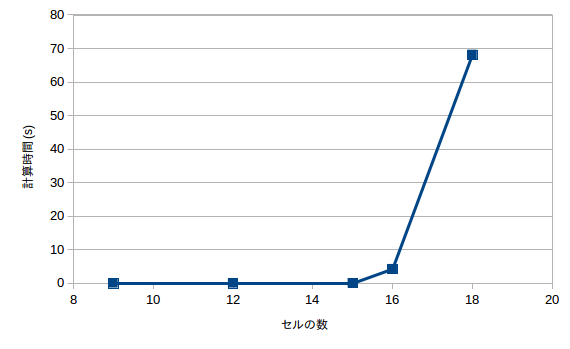
\includegraphics[keepaspectratio, width=90mm]
   {Graphics/chapter3/calTime.png}
   \caption{最適化問題の求解にかかる時間}
   \label{fig:3_3_3_1}
  \end{figure}
  図\ref{fig:3_3_3_1}はセルの数の増加に伴う,最適問題を解くのにかかる時間の変化を表す図である.
開発環境は,OSはUbuntu 16.04,CPUはIntel(R) Core(TM) i7-3770 CPU @ 3.40GHz,メモリは4GBである.
開発言語はR,ソルバーはlpsolveである.
図を見ると,計算時間が指数オーダーで増加していることが確認できる.
$N=20$のときは,計算に5分かかった時点でプログラムの実行を中止した.

  \subsection{実装結果}
  \label{sec:3_3_2}
最後に,ソフトウェア上に実装した結果を示す.
タクシーの時速は60km/hと仮定する.
1単位時間は2分とした.
タクシーは1単位時間で2km進むので,一辺の長さ2kmの正方形のセルを使って対象領域を分割した.
対象領域は大阪駅から堺市あたりまでとした場合,東西に6セル,南北に4セルに分割された(N=24).
過去の乗降車データからは乗車率$\alpha_i$を推定できないため,乗務員の経験則からすべてのセルにおいて乗車率$\alpha_i=0.9$とした.
2単位時間区間(T=2)でモデル予測制御により最適移動分布を計算した.
推奨される走行方向は最適移動分布の中でもっとも大きい値を持つ方向とした.
\begin{figure}[t]
  \begin{minipage}[b]{0.24\linewidth}
    \centering
    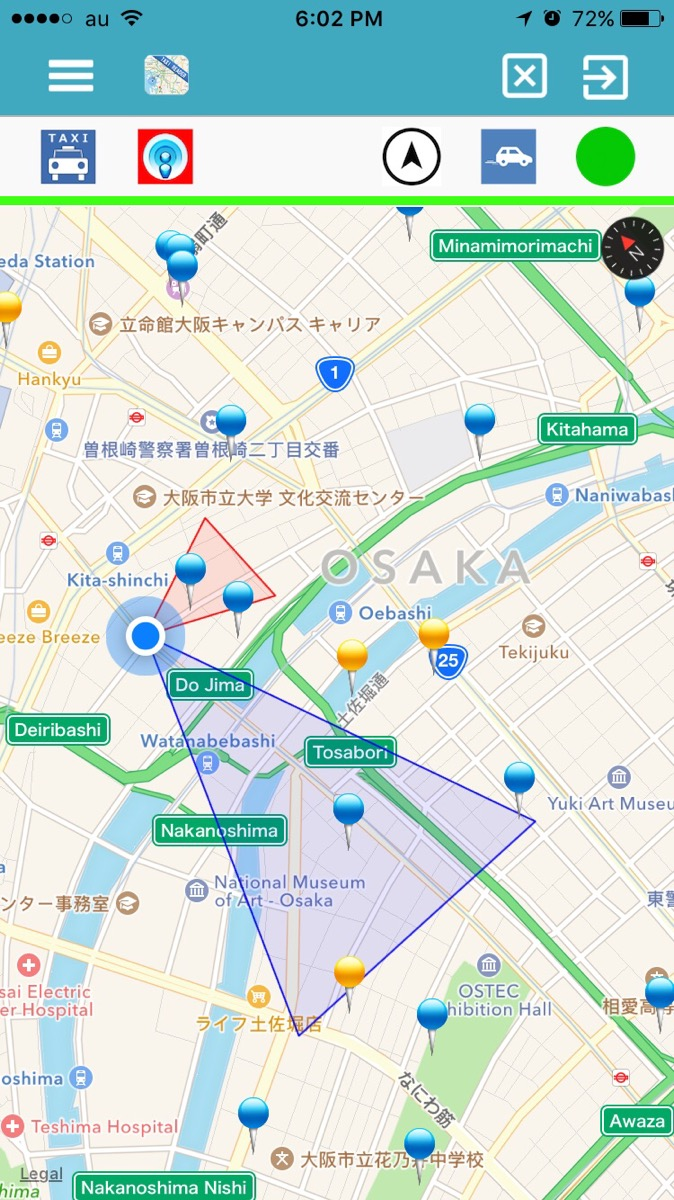
\includegraphics[keepaspectratio, width=22mm]{Graphics/chapter3/201603311802.jpg}
    \subcaption{18時2分}\label{fig:fig3_3_2_1}
  \end{minipage}
  \begin{minipage}[b]{0.24\linewidth}
    \centering
    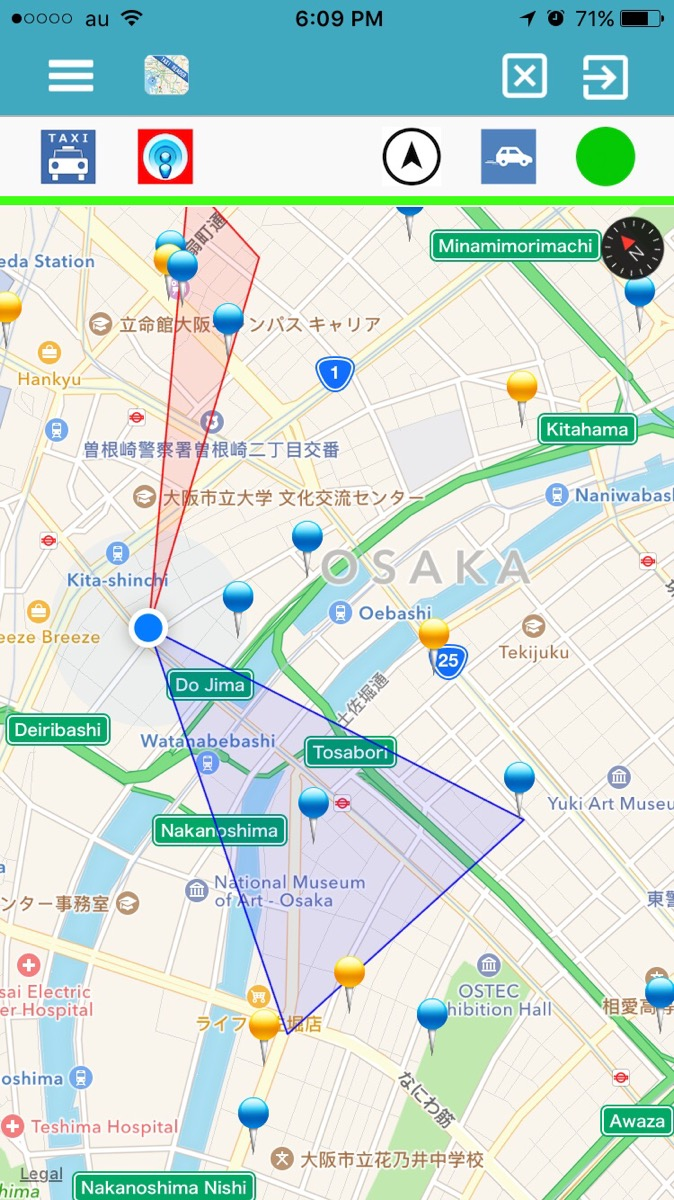
\includegraphics[keepaspectratio, width=22mm]{Graphics/chapter3/201603311809.jpg}
    \subcaption{18時9分}\label{fig:fig3_3_2_2}
  \end{minipage}
  \begin{minipage}[b]{0.24\linewidth}
    \centering
    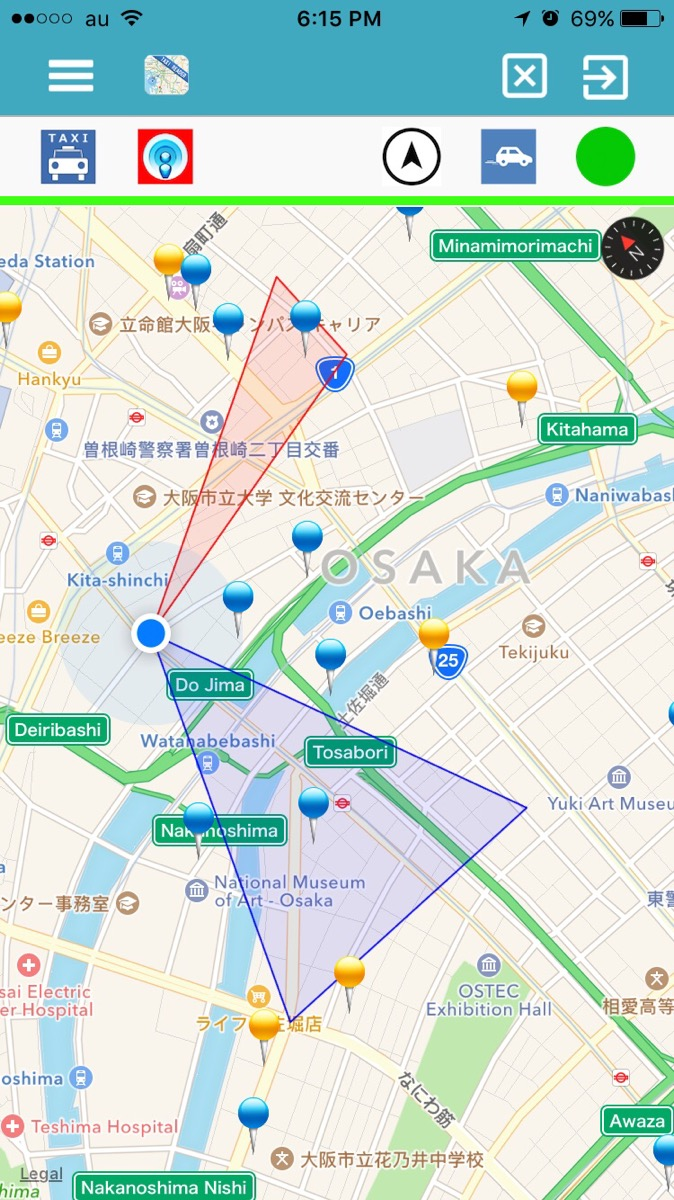
\includegraphics[keepaspectratio, width=22mm]{Graphics/chapter3/201603311815.jpg}
    \subcaption{18時15分}\label{fig:fig3_3_2_3}
  \end{minipage}
  \begin{minipage}[b]{0.24\linewidth}
    \centering
    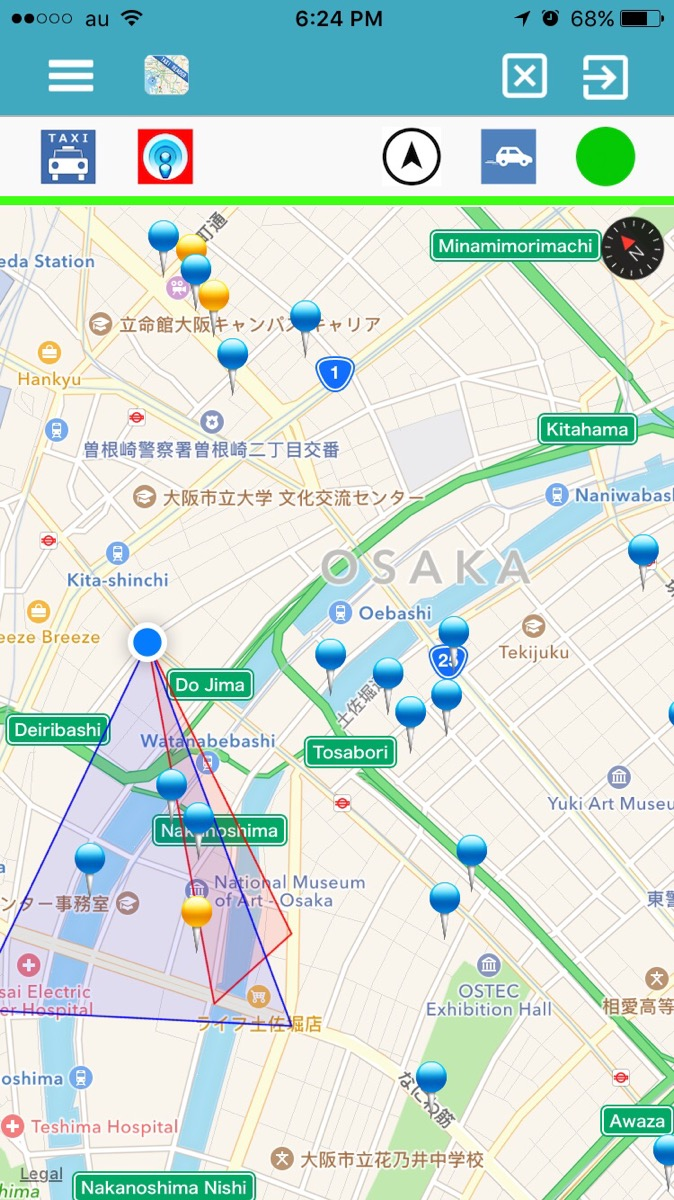
\includegraphics[keepaspectratio, width=22mm]{Graphics/chapter3/201603311824.jpg}
    \subcaption{18時24分}\label{fig:fig3_3_2_4}
  \end{minipage}
  \caption{最適方向の時間的変化(2016年3月31日)}\label{fig:fig3_3_2}
\end{figure}
図\ref{fig:fig3_3_2}に運転手に提示する画面の時間変化を示す.
青色の方向が推奨する最適な方向,すなわち,最適化問題を解くことで得られた,移動するタクシー数が最大となる方向である.
ピンは,現在の日付から2,3,4週間前の日の,現在の時刻から2分前から4分後までの間に乗車実績のあった箇所を表示している.
1辺の長さ200mの正方形のセルで分割された対象領域の,3km範囲内のセルの中で最も乗車数が多いセルを赤色の方向(以下,利己的な方向と呼ぶ)が示している.
18時2分から15分までは,推奨されるな方向と利己的な方向が異なっており,18時24分にはほぼ同じ方向を示している.
最多乗車データのある領域セルが必ずしも最適な方向であるとは限らないことがわかる.
これは,最多乗車データのあるセル周辺に多くの空車タクシーがいる場合には,むしろタクシーを分散させて,対象領域全体として乗客の獲得を図るような最適移動分布を求めているためである.

%  \section{結言}
%  \label{sec:3_4}
%  \par
%  本章では,流しのタクシーの走行支援を目的とした最適移動分布を求める方法を提案した.
% 対象領域をいくつかの分割領域(セル)に分割し,各セル間のタクシーの移動を表すマクロモデルを混合論理動的システムを用いて表し,モデル予測制御によって最適な移動分布を求めた.
% 大阪駅から難波までを対象領域として実データをもとに最適な移動方向分布を計算した結果を示した.
% 乗客数が多いと予想される方向と最も好ましい移動方向とが必ずしも一致しなかった.
% このことから,対象領域全体の予測乗客分布と流しのタクシーの現在の分布をもとにして支援を行うことが重要であることがわかる.

% \par
% 今回の実験では,各セルの一辺の長さを2kmとした.
% また,1時間単位に進むことができるセルは隣接するセルのみとした.
% 長さを短くし,隣接するセル以外にも空車が移動できるようにすれば,より精度よく最適移動方向を計算できるが,計算時間が急速に増大する.
% 計算の並列化,最適解の近似などによる計算時間の短縮が,今後の研究課題である.

 \end{document}
% 結論
%卒業論文用雛形
\documentclass[a4j,12pt,oneside,openany]{jsbook}
% 英語なら以下を使う.
%\documentclass[a4j,12pt,oneside,openany,english]{jsbook}

\usepackage[dvipdfmx]{graphicx}
\usepackage{amssymb}
\usepackage{amsmath}
\usepackage{latexsym}

%jsbook を report っぽくするスタイルファイル
\usepackage{book2report}
%定理,補題,系,例題,証明などや英語用の定義がされています.
%自分なりにいじってください.
\usepackage{thesis}
% 具体的には以下のように定義されています.
% 英語の定理環境
%  \newtheorem{theorem}{Theorem}[chapter]
%  \newtheorem{lemma}{Lemma}[chapter]
%  \newtheorem{proposition}{Proposition}[chapter]
%  \newtheorem{corollary}{Corollary}[chapter]
%  \newtheorem{definition}{Definition}[chapter]
%  \newtheorem{example}{Example}[chapter]
%  \newtheorem{proof}{Proof}
% 日本語の定理環境
%  \newtheorem{theorem}{定理}[chapter]
%  \newtheorem{lemma}{補題}[chapter]
%  \newtheorem{proposition}{命題}[chapter]
%  \newtheorem{corollary}{系}[chapter]
%  \newtheorem{definition}{定義}[chapter]
%  \newtheorem{example}{例}[chapter]
%  \newtheorem{proof}{証明}
% 証明には番号をつけず,最後は Box で終わります.

% 英語で,見出しのフォントが気に入らなかったら
%\renewcommand{\headfont}{\bfseries}

% ページ数が少ないときはここを大きくしてごまかそう!!効果絶大!!
\renewcommand{\baselinestretch}{1.0}

\begin{document}
\chapter{結論}
\label{ch:5}
 \par
 あ
 \end{document}

% 謝辞
%卒業論文用雛形
\documentclass[a4j,12pt,oneside,openany]{jsbook}
% 英語なら以下を使う.
%\documentclass[a4j,12pt,oneside,openany,english]{jsbook}

\usepackage[dvipdfmx]{graphicx}
\usepackage{amssymb}
\usepackage{amsmath}
\usepackage{latexsym}

%jsbook を report っぽくするスタイルファイル
\usepackage{book2report}
%定理,補題,系,例題,証明などや英語用の定義がされています.
%自分なりにいじってください.
\usepackage{thesis}
% 具体的には以下のように定義されています.
% 英語の定理環境
%  \newtheorem{theorem}{Theorem}[chapter]
%  \newtheorem{lemma}{Lemma}[chapter]
%  \newtheorem{proposition}{Proposition}[chapter]
%  \newtheorem{corollary}{Corollary}[chapter]
%  \newtheorem{definition}{Definition}[chapter]
%  \newtheorem{example}{Example}[chapter]
%  \newtheorem{proof}{Proof}
% 日本語の定理環境
%  \newtheorem{theorem}{定理}[chapter]
%  \newtheorem{lemma}{補題}[chapter]
%  \newtheorem{proposition}{命題}[chapter]
%  \newtheorem{corollary}{系}[chapter]
%  \newtheorem{definition}{定義}[chapter]
%  \newtheorem{example}{例}[chapter]
%  \newtheorem{proof}{証明}
% 証明には番号をつけず,最後は Box で終わります.

% 英語で,見出しのフォントが気に入らなかったら
%\renewcommand{\headfont}{\bfseries}

% ページ数が少ないときはここを大きくしてごまかそう!!効果絶大!!
\renewcommand{\baselinestretch}{1.0}

\begin{document}
\begin{acknowledgement}
ありがとう
\end{acknowledgement}

\end{document}

% 参考文献
% 1. 直接書く
\begin{thebibliography}{99}
\bibitem{bib1} 山本俊行, K. Liu,森川高行, “タクシー配車データのプローブデータとしての活用に関する基礎的分析,” 土木計画学研究・論文集,Vol. 23, No. 4, pp. 863-870, 2006.
\bibitem{bib2} 金月寛彰,服部宏充,“プローブカーデータを利用したタクシードライバーの個人特性の分析とモデル化,” 第29 回人工知能学会全国大会, 演題番号1N4-4, 2015.
\bibitem{bib3} K. Zhao, S. Tarkoma, S. Liu, and H. Vo, “Urban HumaMobility Data Mining: An Overview,” in Proc. 2016 IEEE International Conference on Big Data, 2016.
\bibitem{bib4} K. Zhao, D. Khryashchev, J. Freire, C. Silva, and H. Vo, “Predicting Taxi Demand at High Spatial Resolution: Approaching the Limit of Predictability,” in Proc. 2016 IEEE International Conference on Big Data, 2016.
\bibitem{bib5} K. T. Seow, N. H. Dang, and D.-H. Lee, “A Collaborativ Multiagent Taxi-Dispatch System,” IEEE Trans. Automation Science and Engineering, Vol. 7, No. 3, pp. 607-616 ,2010.
\bibitem{bib6} M. Qu, H. Zhu, J. Liu, G. Liu, and H. Xiong, “A CostEffective Recommender System for Taxi Drivers,” in Proc. 20th International Conference on KDD, pp. 45-54, 2014.
\bibitem{bib7} F. Miao, S. Lin, S. Munir, J. A. Stankovic, H. Huang, D. Zhang, T. He, G. J. Pappas, “Dispatch with Real-Time Sensing Data in Metropolitan Areas - A Receding Horizon Control Approach,” in Proc. International Conference on Cyber-Physical Systems, pp. 100-109, 2015.
\bibitem{bib8} F. Miao, S. Han S. Lin, and G. J. Pappas, “Robust Tax Dispatch under Model Uncertainties,” in Proc. 54th IEEE Conference on Decision and Control, pp. 2816-2821, 2015.
\bibitem{bib9} F. MIao, S. Han, S. Lin, Q. Wang, J. Stankovic, A. Hendawi, D. Zhangm T. He, and G. Pappas, “Data-Driven Robust Taxi Dispatch under Demand Uncertainties,” arXiv:1603.06263, 2016.
\bibitem{bib10} A. Bemporad and M. Morari, “Control of Systems Integratin Logic, Dynamics, and Constraints,” Automatica, Vol.35, No. 3, pp. 407-427, 1999.
\bibitem{bib11} 井村順一,東俊一,増淵泉,ハイブリッドシステムの制御,コロナ社,2014.
\end{thebibliography}

% % 2. bibtexを使う
% \bibliography{myjunsrt}
% \bibliography{refs}

% 付録
%卒業論文用雛形
\documentclass[a4j,12pt,oneside,openany]{jsbook}
% 英語なら以下を使う.
%\documentclass[a4j,12pt,oneside,openany,english]{jsbook}

\usepackage[dvipdfmx]{graphicx}
\usepackage{amssymb}
\usepackage{amsmath}
\usepackage{latexsym}

%jsbook を report っぽくするスタイルファイル
\usepackage{book2report}
%定理,補題,系,例題,証明などや英語用の定義がされています.
%自分なりにいじってください.
\usepackage{thesis}
% 具体的には以下のように定義されています.
% 英語の定理環境
%  \newtheorem{theorem}{Theorem}[chapter]
%  \newtheorem{lemma}{Lemma}[chapter]
%  \newtheorem{proposition}{Proposition}[chapter]
%  \newtheorem{corollary}{Corollary}[chapter]
%  \newtheorem{definition}{Definition}[chapter]
%  \newtheorem{example}{Example}[chapter]
%  \newtheorem{proof}{Proof}
% 日本語の定理環境
%  \newtheorem{theorem}{定理}[chapter]
%  \newtheorem{lemma}{補題}[chapter]
%  \newtheorem{proposition}{命題}[chapter]
%  \newtheorem{corollary}{系}[chapter]
%  \newtheorem{definition}{定義}[chapter]
%  \newtheorem{example}{例}[chapter]
%  \newtheorem{proof}{証明}
% 証明には番号をつけず,最後は Box で終わります.

% 英語で,見出しのフォントが気に入らなかったら
%\renewcommand{\headfont}{\bfseries}

% ページ数が少ないときはここを大きくしてごまかそう!!効果絶大!!
\renewcommand{\baselinestretch}{1.0}

\begin{document}
\appendix
\chapter{hoge}
\end{document}

% 研究業績
%卒業論文用雛形
\documentclass[a4j,12pt,oneside,openany]{jsbook}
% 英語なら以下を使う.
%\documentclass[a4j,12pt,oneside,openany,english]{jsbook}

\usepackage[dvipdfmx]{graphicx}
\usepackage{amssymb}
\usepackage{amsmath}
\usepackage{latexsym}

%jsbook を report っぽくするスタイルファイル
\usepackage{book2report}
%定理,補題,系,例題,証明などや英語用の定義がされています.
%自分なりにいじってください.
\usepackage{thesis}
% 具体的には以下のように定義されています.
% 英語の定理環境
%  \newtheorem{theorem}{Theorem}[chapter]
%  \newtheorem{lemma}{Lemma}[chapter]
%  \newtheorem{proposition}{Proposition}[chapter]
%  \newtheorem{corollary}{Corollary}[chapter]
%  \newtheorem{definition}{Definition}[chapter]
%  \newtheorem{example}{Example}[chapter]
%  \newtheorem{proof}{Proof}
% 日本語の定理環境
%  \newtheorem{theorem}{定理}[chapter]
%  \newtheorem{lemma}{補題}[chapter]
%  \newtheorem{proposition}{命題}[chapter]
%  \newtheorem{corollary}{系}[chapter]
%  \newtheorem{definition}{定義}[chapter]
%  \newtheorem{example}{例}[chapter]
%  \newtheorem{proof}{証明}
% 証明には番号をつけず,最後は Box で終わります.

% 英語で,見出しのフォントが気に入らなかったら
%\renewcommand{\headfont}{\bfseries}

% ページ数が少ないときはここを大きくしてごまかそう!!効果絶大!!
\renewcommand{\baselinestretch}{1.0}

\begin{document}
\chapter*{研究業績}
\section*{国際会議}
\begin{itemize}
\item Masaki Hiromoto and Toshimitsu Ushio, ``Learning an Optimal Control Policy for a Markov Decision Process Under Linear Temporal Logic Specifications,''in Proceedings of 2015 IEEE Symposium on Adaptive Dynamic Programming and Reinforcement Learning (in 2015 IEEE Symposium Series on Computational Intelligence), Cape Town, South Africa, pp. 548-555, Dec. 2015.
\item Toshimitsu Ushio, Masaki Hiromoto, Akiyoshi Okamoto, and Tomoaki Akiyama, ``WIP Abstract: A Mixed Logical Dynamical System Model for Taxi Cruising Support System,'' In Proceedings of 2016 ACM/IEEE 7th International Conference on Cyber-Physical Systems Vienna, Austria April 2016.
\end{itemize}
\section*{国内会議}
\begin{itemize}
\item 広本 将基,潮 俊光,「LTL制約の下でのMDPに対するスーパバイザの強化学習」,2016年電子情報通信学会総合大会,p. 166, 2016.
\item 広本 将基,潮 俊光,岡本 明義,秋山 友昭,「モデル予測制御によるタクシーの最適配車問題の定式化」,電子情報通信学会技術報告書,MSS2016-76, SS2016-55, pp. 113-116, 2017.
\end{itemize}
\end{document}

\end{document}

